\section{Changes to the data model}

Due to requirements imposed by the designer, several changes and additions have
been made to the data model. Most of these changes are related to the additional
support for hierarchical networks in the designer. This section present an overview
of new and modified classes and functions.

\subsection{XMASNetwork}

XMASNetwork is a new class designed to represent an xMAS network. This class can be
used to model both flat and hierarchical networks. When used to model hierarchical
networks, an XMASNetwork represents a single level or subnetwork in the hierarchy.
Multiple networks are combined to form the complete network.

The main responsibility of XMASNetwork is to serve as a container of XMASComponent
instances. Internally, XMASNetwork stores the components in a map relating a
components name to its in-memory instance. Prior to the introduction of XMASNetwork,
the concept of an xMAS network was directly represented by such a map. Verification
tools still use this approach, although they could be easily adapted to use
XMASNetwork as well.

\paragraph{}
The 'promotion' of XMASNetwork to its own class definition has two primary reasons:
\begin{itemize}
 \item The designer uses additional network properties like the canvas size. These
 properties must be stored somewhere in the data model (i.e. in XMASNetwork).
 \item Support for hierarchical networks requires management of multiple network
 models. Using an explicit class to represent networks eases this task.
\end{itemize}

\paragraph{Extending networks}
XMASNetwork implements the same extension mechanism as used by the XMASComponent and
Port classes. For this, a new class named XMASNetworkExtension has been created.
Currently, the designer uses two network extensions. One to store network
properties common to all models, and one to store network properties specifically
for network models that are to be used as composite objects.
In the future, additional network extensions could be defined, for example to store
data required to support parameterization of subnetworks.

\paragraph{MemoryPool}
All components in an XMASNetwork are stored in a MemoryPool for optimal performance.
Multiple networks can share a MemoryPool instance. The XMASNetwork constructors
optionally take a pointer to a MemoryPool. Passing the same instance to multiple
networks will let these networks share the pool. When no MemoryPool pointer (or
nullptr) is provided to the constructor, XMASNetwork will create its own
MemoryPool instance. In this case, XMASNetwork also takes care of the MemoryPool
destruction.


\subsection{XMASComposite}

When modeling a hierarchical network, composite objects are used to represent
subnetworks as black boxes inside a higher-level network. The addition of
composite objects to an xMAS network is reflected in the data model through the
new XMASComposite class. Like the eight xMAS primitive types, XMASComposite
is derived from XMASComponent. As such, XMASComposites can be used in the same
way as the primitive components.

When a new XMASComposite object is created, a reference to an XMASNetwork must
be passed to the constructor. The composite object will represent an
instantiation of this (sub)network.

The sinks and sources of the subnetwork are used as interface ports or gates
between the subnetwork and the higher-level network. An xMAS source component
will result in an Input port on the composite object. Likewise, each xMAS sink
component in the subnetwork leads to an Output port on the composite object.

\subsubsection{Hierarchical visitors}

Due to the introduction of the new XMASComposite type, the XMASComponentVisitor
interface has been extended to support composite objects. Unlike the existing
pure virtual visit functions, XMASComponentVisitor provides a default
implementation to visit XMASComposites. This way, existing implementations of
the interface which weren't designed to support composites aren't affected. The
default visit implementation for composite objects does throw an Exception however.
So, only flat, composite free networks should be passed to these implementations.


\subsection{XMASProject}

The xMAS designer application uses the XMASProject class to manage a complete
hierarchical model. The root network, available through getRootNetwork(), is
the network under construction. For each composite object type used, XMASProject
additionally stores its network definition. XMASProject is equipped with member
functions to insert new components into the network, remove them from the network
and change the name of a component. All of these functions act upon the root network.
Adding a new composite object to the model requires that its network definition
is added to the project in advance. Function insertComposite() automatically does
this if necessary. A subnetwork that is no longer of use can be unloaded using
unloadNetwork(). Unloading only succeeds if no composite objects in the project
(at any level) depend on the network.

XMASProject is also responsible for the construction and destruction of a MemoryPool.
All networks loaded in the project share this instance of the pool.

\paragraph{Note:}
Currently, the designer assumes that all subnetworks used in a project are
stored in the same directory as the root network.

\begin{figure}
    \centering
    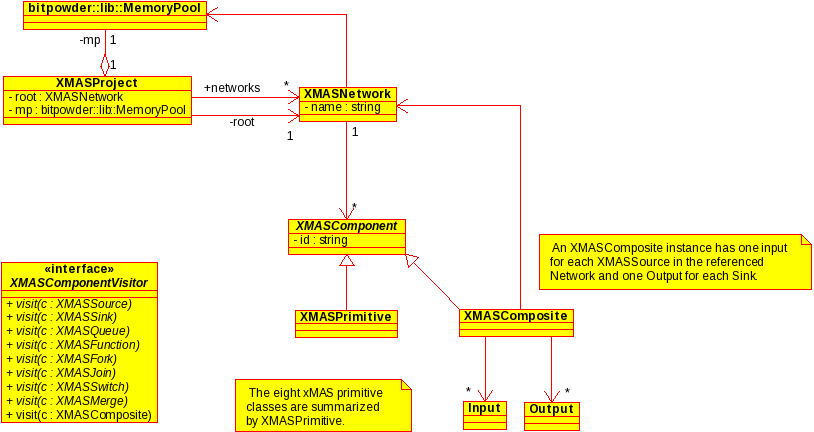
\includegraphics[width=0.8\textwidth]{new-xmas-datamodel}
    \caption{xMAS data-model extended with new classes}
\end{figure}


\subsection{Parser \& Exporter}

The additional support for hierarchical models and the need to store data used
by the designer require a number of modifications to the parser and the exporter.

\paragraph{Position}
For each component listed in the json data, the parser checks whether canvas data
is available in the pos field (see also the file format description). If this is
indeed the case, the x, y, orientation and scale fields are read and stored inside
an extension of the component (CanvasComponentExtension). If no position data
is stored in the json data, the designer will use default values. The exporter has
been updated to write the position data, if present, back to json as well.

\paragraph{Composite objects}
XMASComposite objects are created for all components in the json file with type
'composite'. The parser uses the 'subnetwork' attribute mandatory for composite
components to determine what kind of composite object should be created. The
parser is not responsible for loading subnetworks. Rather, the caller of the parser
must supply a function that is able to map a subnetwork name to an instance of
an XMASNetwork. Code that uses the parser should be updated to comply with the
new function signature. The implementation in XMASProject can be used as a reference.


\newpage

